\documentclass{scrreprt}
\usepackage{listings}
\usepackage{underscore}
\usepackage{graphicx}
\usepackage[bookmarks=true]{hyperref}
\usepackage[utf8]{inputenc}
\usepackage[english]{babel}
\usepackage{fancyhdr}
\usepackage{hyperref}
\usepackage{graphicx}

\hypersetup{
    bookmarks=false,    % show bookmarks bar?
    pdftitle={Software Requirement Specification},    % title
    pdfauthor={},                     % author
    pdfsubject={TeX and LaTeX},                        % subject of the document
    pdfkeywords={TeX, LaTeX, graphics, images}, % list of keywords
    colorlinks=true,       % false: boxed links; true: colored links
    linkcolor=blue,       % color of internal links
    citecolor=blue,       % color of links to bibliography
    filecolor=black,        % color of file links
    urlcolor=blue,        % color of external links
    linktoc=page            % only page is linked
}%
\def\myversion{1.0 }
\date{}
%\title



\renewcommand{\headrulewidth}{2pt}
\renewcommand{\footrulewidth}{1pt}
\begin{document}
\begin{titlepage}
\topskip0pt
\vspace*{\fill}
\begin{center}

    \Huge{\textbf{Team_555}}
\end{center}

\vspace*{\fill}
  
\end{titlepage}
\cleardoublepage
\begin{flushright}
    \rule{16cm}{5pt}\vskip1cm
    \begin{bfseries}
        \Huge{SOFTWARE REQUIREMENTS\\ SPECIFICATION}\\
        \vspace{1.5cm}
        \vspace{1.5cm}
        
        \vspace{1.5cm}
      \today\\
        \vspace{1.5cm}
        \vspace{1.5cm}
        \vspace{1.5cm}
        
    \end{bfseries}
\end{flushright}

\tableofcontents

\chapter{. Introduction}

\section{Purpose}
The purpose of the Online Food Ordering System\textbf{(Anytime food app)} is to automate the existing manual system by the help of computerized equipments and full-fledged computer software,fulfilling their requirements,so that their valuable data/information can be stored for a longer period with easy accessing and manipulation of the same.\\ \\
The key catalyst of this project is also to increase convenience and transparency for both the ends i.e. customers as well as merchants.It also helps to avoid human error and delay for scheduling tasks.\\ \\
The online food-delivery has already seen much growth in the past few years,but now online food-deliveries are much in demand due to social distancing.\\ \\
This app make easy for user to buy product
from store with easy steps and store can get easy order.


\section{Project Scope}
The given Problem Statement is very detailed, discrete and specific. It requires us to build a Restaurant app which can be used by common people to order food. \\ \\
In this report, we gloss over the functionalities of the App and major technologies used, so as to understand the significance of each component. We have extensively used Kubernetes which provides an authentic consumer experience even during a downtime at its centralized IT core. \\

\chapter{. Overall Description}
The following section presents an overall description of the subject. In particular, the product
has been put into perspective through a detailed assessment of the system, user, hardware, software
and communication interfaces, memory considerations, operational modes and site adaptation
requirements. Further, characteristics of the system’s end-users are discussed along with the
identified system constraints and assumptions. To conclude the section, an apportioning of
requirements has been outlined.

\section{Product Perspective}
Anytime food application enables a user to place the order of food item he wishes. This application will also help the customer to view his previous orders and their regarding values.The user can also just add an item to cart without placing the order ,so that he can order it in future.
User can also edit his profile details in the dashboard.




\section{Product Functions}
\subsection{The Web Ordering System:}
Users of the web ordering system namely restaurant customers, must be provided the following functionality: \\ \\
• Login Functionality - through Username and Password \\
• Creation of User Account \\
• Management of Accounts - Editable Password and Username \\
• Local storage of User Information - Address, Phone Number, Password and Username \\
• Navigate the restaurants menu.\\
• Select an item from the menu.\\
• Customize options for a selected item.\\
• Add an item to their current order.\\
• Review their current order.\\
• Remove an item/remove all items from their current order.\\
• Provide delivery and payment details.\\
• Place an order.\\
• Receive confirmation in the form of an order number.\\
\newline
As the goal of the system is to make the process of placing an order as simple as possible for the customer, the functionality provided through the web ordering system is restricted to to that which most pertinent to accomplish the desired task. All of the functions outlined above with the exceptions of account creation and management will be used every time a customer places an order. \\
\newline
\subsection{Menu Management System:} 
The menu management system will be available only to restaurant employees and as the name suggests allows them to manage the menu that is displayed to users of the web ordering system.The functions afforded by the menu management system provide user with the ability to using a graphical interface. \\ \\
• Add a new/update/delete vendor to/from the menu. \\
• Add a new/update/delete food category to/from the menu.\\
• Add a new/update/delete food item to/from the menu.\\
• Add a new/update/delete option for a given food item.\\
• Update price for a given food item.\\
• Update default options for a given food item.\\
• Update additional information(description, photo etc.,) for a given food item.\\

\subsection{Order Retrieval System:}

Of the three components the order retrieval system is functionally the simplest.Like the menu management system it is designed to be used only by restaurant employees and provides the following functions given below: \\ \\
• Retrieve new orders from the database. \\
• Display the orders in an easily readable, graphical way.\\
• Mark an order as having been processed and remove it from the list of active orders.\\
\section{User Interface}
Each of the system components will have their own unique interface. These are described below. \\  \\
\textbf{Web Ordering System:}
Users of the web ordering system will interact with the application through a series of simple forms. Each category of food has its own form associated with it which presents a drop down menu for choosing which specific item from the category should be added to the order. Adding an item to the order is accomplished by a single button click. Users select which category of food they would like to order and therefore which form should be displayed by navigating a menubar, an approach which should be familiar to most users. \\ \\
\textbf{Menu Management System:} 
User interaction with the menu management system is similar to that with the web ordering system.Users navigate a tree structure to find the specific food item that they would like to modify and after making their selection they are presented with a form which displays all of the current fields and values associated with that item, all of which can be modified or removed.The interface also presents buttons which allow the addition of new fields and values.\\ \\
\textbf{Order Retrieval System:}
User interaction with the order retrieval will be very simple. This application will automatically fetch new orders from the database at regular intervals and display the ordernumbers, along with delivery time, in a panel on the left hand side of the application. To view the details of an order, the user must simply click on that order number which will populate the right-hand panel with the details displayed in an easy to read and navigate tree structure. \\

\section{Operating Environment}
The website will be operate in any Operating Environment - Mac, Windows, Linux etc... 

\section{Description of the Core Technologies Used}
In our solution design, we have used various technologies for various sub-problems. We believe that before we go on to explain our solution, it is important for the reader to understand the core technologies beforehand, and to get the gist of what we are trying to do, and to understand the importance of each sub-steps as to why they are important. \\


\subsubsection{\textbf{React Native:}}
React Native apps perform almost exactly like a native app that was built on the specific iOS or Android platform. They are also fast because the programming language is optimized for mobile devices. Instead of mainly using the central processing unit (CPU), React Native apps take advantage of the graphics processing unit (GPU). This makes them much faster than cross-platform hybrid technologies.\\ \\
Similar to React for the Web, React Native applications are written using a mixture of JavaScript and XML-esque markup, known as JSX. Then, under the hood, the React Native “bridge” invokes the native rendering APIs in Objective-C (for iOS) or Java (for Android). Thus, your application will render using real mobile UI components, not webviews, and will look and feel like any other mobile application. React Native also exposes JavaScript interfaces for platform APIs, so your React Native apps can access platform features like the phone camera, or the user’s location. \\


\subsubsection{\textbf{Node js:}}
It is a server-side JavaScript platform using an event-driven, non-blocking I/O model allowing users to build fast and scalable data-intensive applications running in real time.Node js interprets JavaScript code through Google’s V8 JavaScript engine that directly compiles JavaScript code into machine code. \\

\subsubsection{\textbf{Kubernetes:}}	
First developed by Google, Kubernetes is an open-source orchestrator for deploying containerized applications in a clustered environment. Kubernetes allows DevOps teams to automate container provisioning, networking, load balancing, security, and scaling across a cluster.

\subsubsection{\textbf{Docker:}}	
It is a container runtime platform, that helps to containerise applications, with just a few commands (or using Docker UI buttons). It helps to build Docker images (which are the templates for the containers to run), and upon running these images, the containers are created and run on the Host OS. It can also seamlessly delete these containers or images, as and when required.

\subsubsection{\textbf{Amazon Web Services (AWS):}}	
It provides cloud services (depending upon our requirements), and the services cost differently, based on the pricing model and the service, and the no. of instances created, resources used, etc. It is one of the leading cloud service providers.
    Many services are provided by AWS. Out of these, we are using - 
a. Elastic Container Registry (ECR) Service: The Docker Images are hosted on instances of this service
b. Relational Database Service (RDS): The SQL Database is hosted on instance of this service
c. Elastic Kubernetes Service (EKS): To host Kubernetes and its config files (.yaml) and run the containerised application in microservices architecture

\chapter{. System Features}

\section{Description and Priority}
The online web application has features that are main and also some are sub. But all the feature is necessary for this software.
\newline
The features are given below - 
\begin{enumerate}
\item Easy Order Placement: Most of the people prefer to order online because the order placement process is quick and simple. This is only possible if your app has been designed from a friendly usability perspective. On-demand food delivery app must have a great user interface (UI) design. A user interface is an essential part of the app through which users communicate with the app and order services. \\

The users should have the option to effectively explore and discover what they need. If the UI is taking time to load, the user experience will be affected. Thus it is considered as one of the most significant components of the app for its progress. It must load all the elements very quickly for great user experience with better app engagement and conversion rate.
    \item Easy Payment Options :Though it’s the last process of the order placement if a customer faces any minor/major problem they won’t ever try again. So, making the payment procedure exceedingly productive and simple to use, a customer must have all the payment options listed in your on-demand food delivery app.
    \item Reviews & Ratings: This is a well tested and great way for businesses to know how customers are responding to their app. If your app is rated well, then the chances are high that lots of people will prefer visiting your app. Therefore, adding a feedback portal would help your business to get instant and quick bites of knowledge so that you get insights into what amendments to be made in your app in the future for better customer experience.
    \item Search Filters: Customers will appreciate the ease and time savings that a sophisticated search feature with numerous criteria may provide as You have the freedom to search out the eateries you want by downloading a restaurant aggregator/ordering app. Accordingly, users should search for items based on timely delivery, distances, or even menu choices, which vary from place to More is required for an app for a single restaurant or chain.
    \item Order History: The user must be able to see his history of orders along with the expenditure. 

\end{enumerate}

\section{Functional Requirements}
 These are requirements that must be met, and cannot be done without. As a development contract, these requirements need to be clearly stated and documented before the development begins. They must be recorded as inputs that must be given to the system, before the operation is processed and output is delivered to the user.\\

Some examples of functional requirements would include: 
\begin{enumerate}
    \item \textbf{Authentication:} The Anytimefood app deploys login functionality UI and APIs, to post the user data (Name and Password) into database, that helps each user to login using their names and passwords. This information along with their phone numbers and addresses are also stored locally in his/her machine.
    \item \textbf{Business core:} 
    \begin{itemize}
        \item Food Delivery Time: We deliver food very quickly. This is due to the fast response of the Food Delivery Team, and also attributed to the backend microservices and load balancing architecture. The user orders are posted on the database using API calls and the routing load is balanced using Ingress Controller Nginx. This ensures that even if too many clients post orders at the same time, the server instances would not be overloaded, and new containers can be created to take some of the routes. So, the order posting time to the database, accessible by the restaurant members will be fast, and we can quickly assign the orders to the delivery teams.
        \item Simple User Interface: We provide a Simple UI to help customers quickly identify the features and requirements of the food delivery app. It would promote our application very quickly among users.
        \item Prevention of Downtime of Servers: Due to the microservices architecture implemented in cloud, our Application will hardly ever give a tough time to the users. If any of the service container fails, our kubernetes config files ensure that a new one is immediately deployed in the proper nodes. This will ensure that the servers would keep running, and users would hardly face any issue with the app, due to server failure.
    \end{itemize}
    \item \textbf{Transactions and Checkouts:}  The Cart page shows all the pricing of the items ordered by the users, and their quantities, and the total price. The user can then finalise the order and will be directed to the Checkout page, to get the documented transaction page.
    \item \textbf{Historical Data: } The Historical Data of the previous orders of all users are stored in the database. So, they can check and access their previous orders with the UI provided.
\end{enumerate}

\chapter{. Other Nonfunctional Requirements}

\section{Performance Requirements}
\begin{itemize}
    \item  The product requires to access and modify multiple databases.\\
    \item The software should not exhibit any signs of deterioration or slow-down in
terms of response time as the user-traffic and scheduling data increases. \\
\item The product’s performance also depends on the hardware components of the
device.\\
\end{itemize}
 


\section{Safety Requirements}
\begin{itemize}
    \item Since the product is a web based application, it has chances of internet risks such
as viruses which the software should be able to minimize \\
\item Online backup in case of server failure\\
\end{itemize}

\section{Security Requirements}
\begin{itemize}
    \item One users data is not accessible through other user.\\
    \item Personal Information of User (Address and Phone Number) is only available, locally, and Username and Password, is stored securely in database.\\

\end{itemize}
\section{Software Quality Attributes}
\begin{itemize}
\item Availability:
The application can be used 24 hours a day,7 days a week. \\

\item Maintainability: Further development of code is possible and various versions can be maintained. It is easy to add additional feature to the software, without downtime and modify it. \\
\item Usability: This software can be easily used by anyone and it also has a help link to guide
users. The interface is itself very user-friendly and the error messages tell you where
you went wrong. \\
\item Robustness:
The software is made to be robust enough to have a high degree of fault tolerance. For
example, the system should not crash if the user enters an invalid input. It should display
a suitable error message. \\
\item Portability:
 The application should be easily deployable and maintainable. \\
\end{itemize}


\section{Business Rules}
The Software should not be used by a third party without prior permission. All rights are
reserved by our Organisation. 

\chapter{. Other Requirements}
Licensing Requirements: Applicable \\
Legal,Copyright and Other Notices: All rights reserved by our Organisation \\
Applicable Standards: It should be as per Industry Standard \\ \\
 \textbf{Database: } The database is hosted on Amazon Web Services (AWS) Relational Database Service (RDS). It will ensure scalability whenever the database grows.\\\\
\textbf{Docker Images: } The Docker Images are pulled from the AWS Elastic Container Registry (ECR) Service.\\\\
\textbf{Kubernetes Cluster: } The Kubernetes Cluster is hosted in AWS Elastic Kuberenetes Service (EKS).



\chapter{. References}
\section*{Technology References:}
\begin{itemize}
    \item  \href{https://reactnative.dev/}{React Native} \\
 \item \href{https://nodejs.org/en/}{Node js} \\
\item \href{https://kubernetes.io/}{Kubernetes} \\
\item \href{https://www.mysql.com/}{MySQL} \\
\item \href{https://www.typescriptlang.org/}{TypeScript} 
\end{itemize}
\newpage
\begin{flushright}
    \rule{16cm}{5pt}\vskip1cm
    \begin{bfseries}
        \Huge{Data Flow and Control Flow Diagrams}\\
        \vspace{1.5cm}
        \vspace{1.5cm}
        
        \vspace{1.5cm}
     \textbf{Prepared By : Team_555}
        \vspace{1.5cm}
        \vspace{1.5cm}
        
    \end{bfseries}
\end{flushright}

\newpage
\section*{Control Flow Diagram:}
\vspace{20pt}
\begin{figure}[h!]
    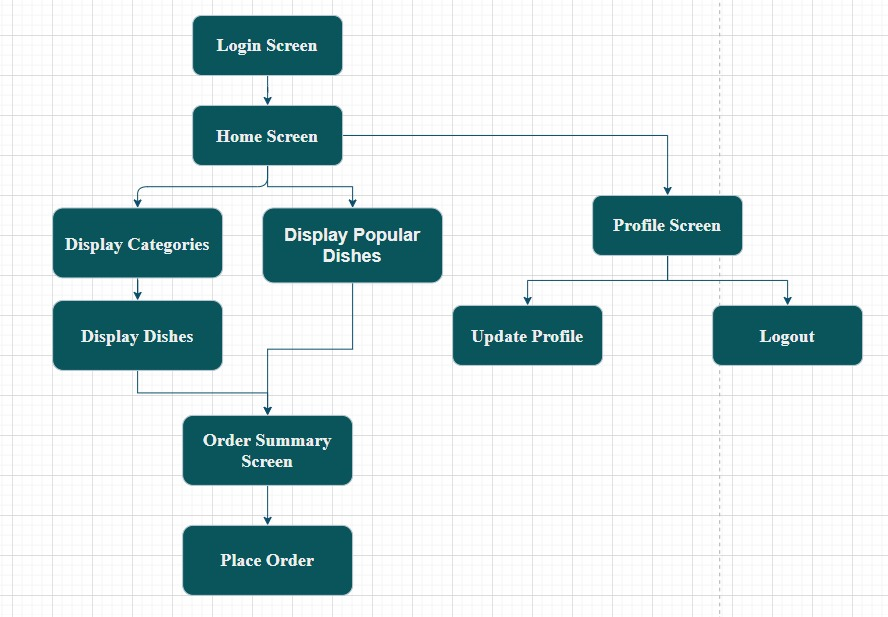
\includegraphics[scale=0.55]{Control_flow.jpeg}
   
    
\end{figure}
\newpage
\section*{Data Flow Diagram:}
\vspace{20pt}
\begin{figure}[h!]
\begin{center}
    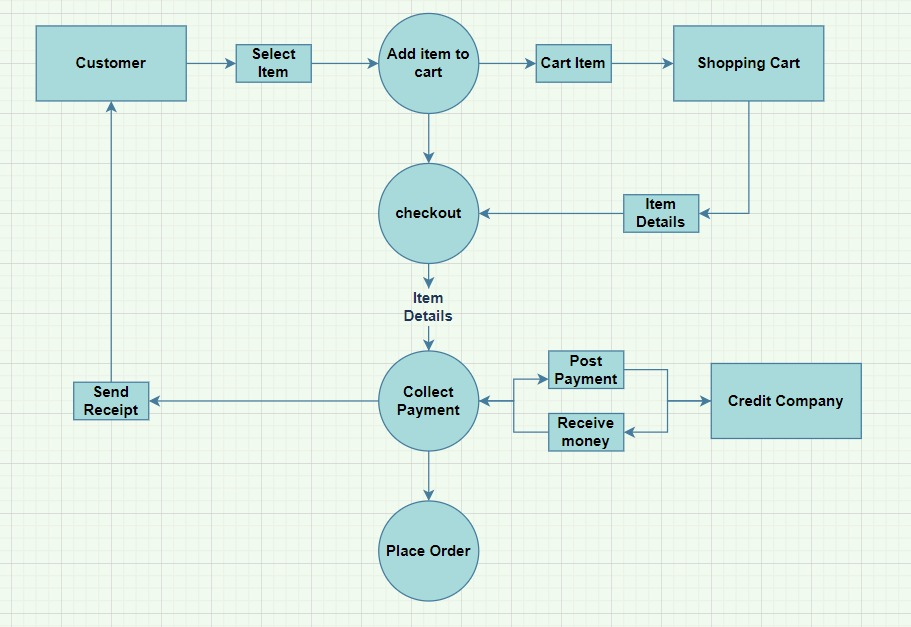
\includegraphics[scale=0.5]{Dataflow.jpeg}
\end{center}
\end{figure}
\newpage
\begin{flushright}
    \rule{16cm}{5pt}\vskip1cm
    \begin{bfseries}
        \Huge{Detailed Design of Class diagrams and relations}\\
        \vspace{1.5cm}
        \vspace{2.5cm}
        
        \vspace{1.5cm}
     {Prepared By : Team_555}
        \vspace{1.5cm}
        \vspace{1.5cm}
        
    \end{bfseries}
\end{flushright}
\newpage
\section*{Class Diagram and relations:}
\vspace{20pt}
\begin{figure}[h!]
    \centering
    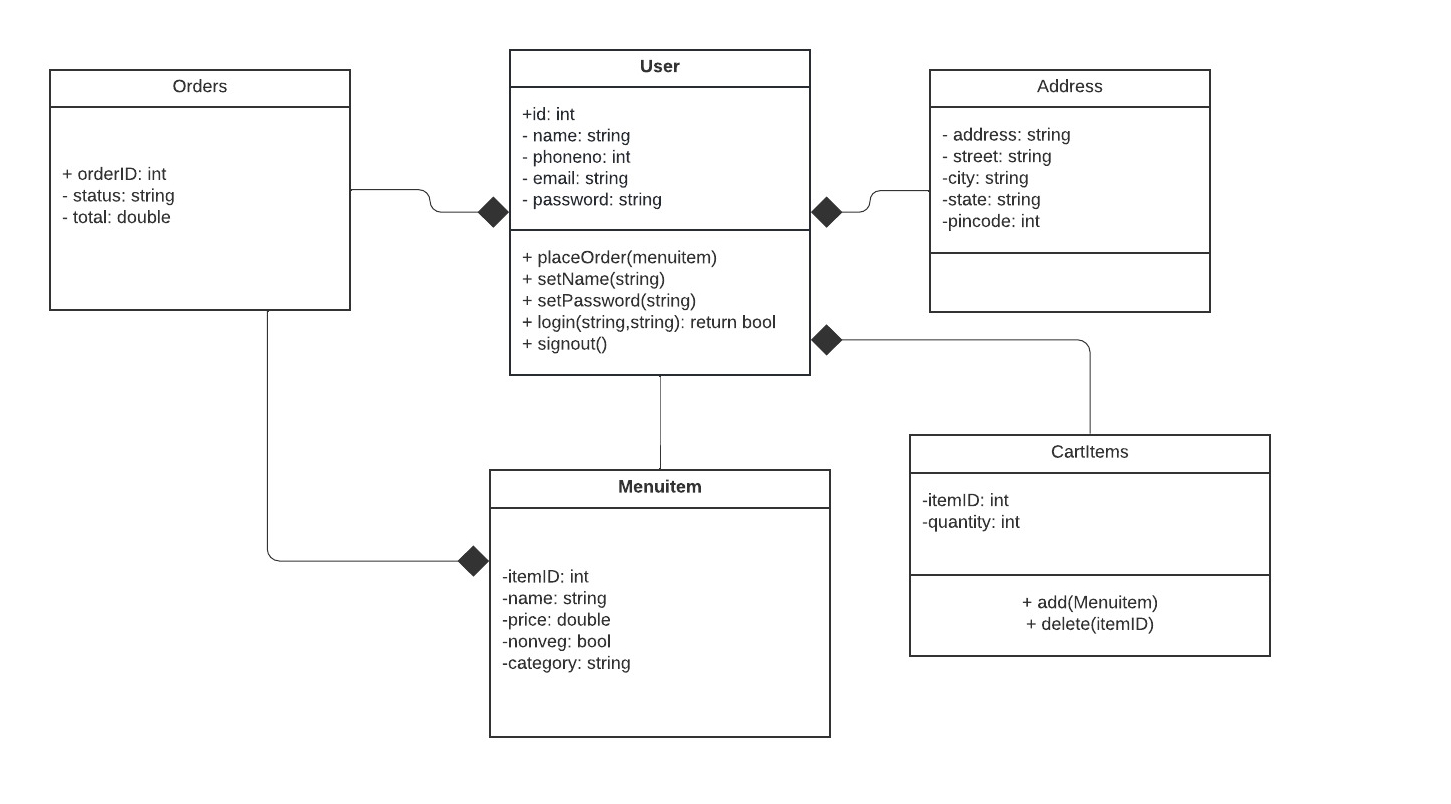
\includegraphics[scale=0.8]{UML class.jpeg}
    
\end{figure}
\newpage
\section*{Database Schema Diagram:}
\begin{figure}[h!]
    \centering
    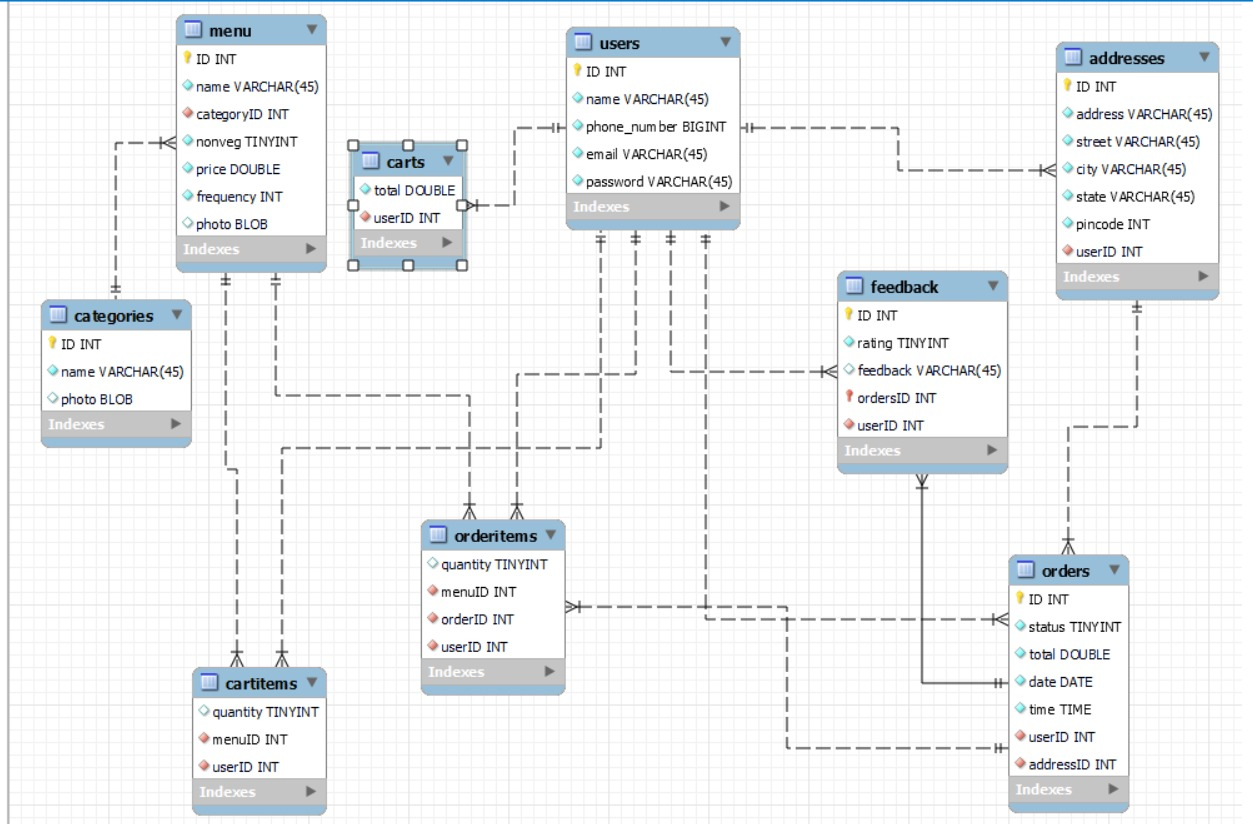
\includegraphics[scale=0.4]{Class_diagram.jpg}
    
\end{figure}
\newpage
\section*{Test Cases Screenshots:}
\begin{figure}[h!]
    \centering
    \includegraphics[scale=0.4]{code.jpg}
    
\end{figure}
\begin{figure}[h!]
    \centering
    \includegraphics[scale=0.4]{error.jpg}
    
\end{figure}
\begin{figure}[h!]
    \centering
    \includegraphics[scale=0.4]{Serverdown.jpg}
    
\end{figure}
\begin{figure}[h!]
    \centering
    \includegraphics[scale=0.4]{IMG-20220331-WA0081.jpg}
    
\end{figure}
\end{document}